\documentclass[tikz]{standalone}
\usepackage{tikz}
\usepackage{helvet} % Lädt das Helvetica-Paket
\renewcommand{\familydefault}{\sfdefault} % Setzt Helvetica als Standardschriftart

\begin{document}

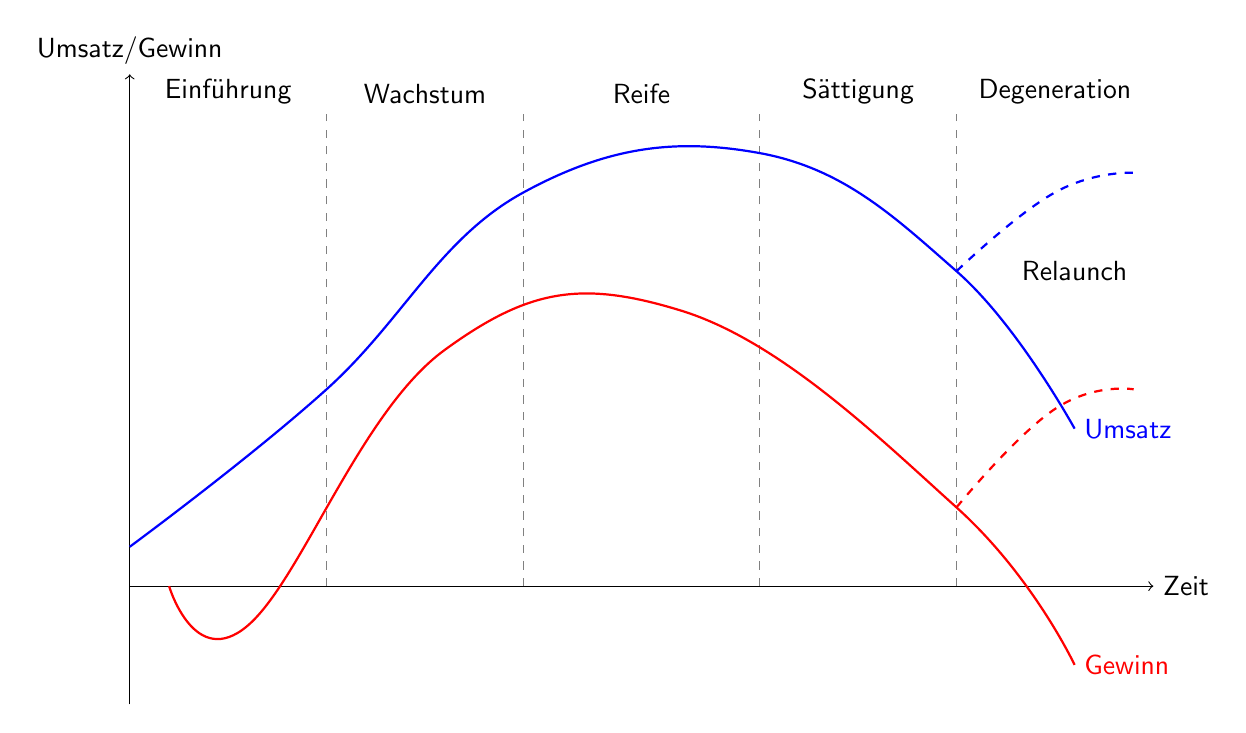
\begin{tikzpicture}
    % --- Achsen ---
    % X-Achse (Zeit)
    \draw[->] (0,0) -- (13,0) node[right] {Zeit};
    % Y-Achse (Umsatz/Gewinn)
    \draw[->] (0,-1.5) -- (0,6.5) node[above] {Umsatz/Gewinn};

    % --- Phasen des Produktlebenszyklus ---
    % Trennlinien und Beschriftungen für die Phasen
    \draw[dashed, gray] (2.5,0) -- (2.5,6);
    \node[above] at (1.25,6) {Einführung};
    \draw[dashed, gray] (5,0) -- (5,6);
    \node[above] at (3.75,6) {Wachstum};
    \draw[dashed, gray] (8,0) -- (8,6);
    \node[above] at (6.5,6) {Reife};
    \draw[dashed, gray] (10.5,0) -- (10.5,6);
    \node[above] at (9.25,6) {Sättigung};
    \node[above] at (11.75,6) {Degeneration};

    % --- Kurvenverläufe ---
    % Umsatzkurve (blau) mit geglättetem Plot
    \draw[blue, thick] plot[smooth, tension=0.7] coordinates {
        (0, 0.5) (2.5, 2.5) (5, 5) (8, 5.5) (10.5, 4) (12, 2)
    };
    \node[blue, right] at (12, 2) {Umsatz};

    % Gewinnkurve (rot) mit geglättetem Plot
    \draw[red, thick] plot[smooth, tension=0.7] coordinates {
        (0.5, 0) (1.5, -0.5) (4, 3) (7, 3.5) (10.5, 1) (12, -1)
    };
    \node[red, right] at (12, -1) {Gewinn};
    
    % --- Relaunch-Kurven ---
    % Relaunch Umsatz (blau, gestrichelt)
    \draw[blue, thick, dashed] plot[smooth, tension=0.8] coordinates {
        (10.5, 4) (11.75, 5) (12.75, 5.25)
    };

    % Relaunch Gewinn (rot, gestrichelt)
    \draw[red, thick, dashed] plot[smooth, tension=0.8] coordinates {
        (10.5, 1) (11.75, 2.25) (12.75, 2.5)
    };
    
    % Beschriftung für Relaunch
    \node at (12, 4) {Relaunch};
\end{tikzpicture}

\end{document}
